% Drawing 148/02-13 -- folder 148, batch 02, archive page 33 (PDF page 34).
% Transcription: à droite, une petite sphère dont l'équateur porte cinq points, trois à l'avant et deux à l'arrière.
% Kind: sphere with five points on the equator. Method 2 (schematic redraw from the facsimile). Status: ok.
% Notes: Ink. The outline, the front of the equator, and five dots: the left end of the equator, two on the front arc, two on the back (which has no drawn line). A short stray arc under the equator is left out. Redrawn 2026-11-12 (issue 128): to check again.
% Coordinates: 1 unit = 1 mm = 1/100 of the crop width, y downwards as on the crop (bbox in page fractions: [0.72, 0.405, 0.86, 0.46]).
% Redrawn by Claude (claude-fable-5-2), issue #128, 2026-11-12; not checked by a human; not compiled (no TeX in the session).
% Rights: reproduces part of the work -- behind RENDER_TRANSCRIPTS, never published by itself.
\documentclass[tikz,border=3pt]{standalone}
\usepackage{amsmath,amssymb}
\usetikzlibrary{patterns,arrows.meta}
\tikzset{pencil/.style={black!45}, struck/.style={black!35}, mpt/.style={circle,draw,inner sep=1.3pt}, pt/.style={circle,fill,inner sep=0.9pt}, opt/.style={circle,draw,fill=white,inner sep=1.1pt}, Rd/.style={red!75!black}, Gn/.style={green!45!black}, Br/.style={brown!70!black}}
\begin{document}
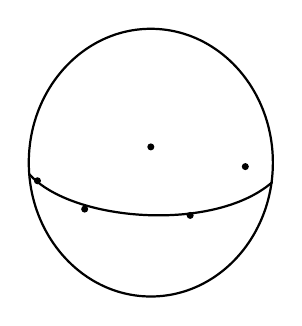
\begin{tikzpicture}[x=1mm,y=-1mm,line cap=round,line join=round,font=\small]
\draw[thick] (36,29.5) ellipse [x radius=15.5, y radius=17];
\draw[thick] (20.6,31) .. controls (26,37) and (44,38.4) .. (51.4,32);
\node[pt] at (21.6,31.8) {};
\node[pt] at (27.6,35.4) {};
\node[pt] at (41,36.2) {};
\node[pt] at (36,27.5) {};
\node[pt] at (48,30) {};
\end{tikzpicture}
\end{document}
